\documentclass[fleqn,10pt]{latex/stylish_article} % Document font size and equations flushed left

\setcounter{tocdepth}{3}

% Pandoc environments
\usepackage{framed}
\usepackage{fancyvrb}
\providecommand{\tightlist}{%
  \setlength{\itemsep}{0pt}\setlength{\parskip}{0pt}}
\newcommand{\VerbBar}{|}
\newcommand{\VERB}{\Verb[commandchars=\\\{\}]}
\DefineVerbatimEnvironment{Highlighting}{Verbatim}{commandchars=\\\{\}, fontsize=\scriptsize} % R Code

% Colored code
\usepackage{color}
\definecolor{shadecolor}{RGB}{248,248,248}
\newenvironment{Shaded}{\begin{snugshade}}{\end{snugshade}}
\newcommand{\KeywordTok}[1]{\textcolor[rgb]{0.13,0.29,0.53}{\textbf{{#1}}}}
\newcommand{\DataTypeTok}[1]{\textcolor[rgb]{0.13,0.29,0.53}{{#1}}}
\newcommand{\DecValTok}[1]{\textcolor[rgb]{0.00,0.00,0.81}{{#1}}}
\newcommand{\BaseNTok}[1]{\textcolor[rgb]{0.00,0.00,0.81}{{#1}}}
\newcommand{\FloatTok}[1]{\textcolor[rgb]{0.00,0.00,0.81}{{#1}}}
\newcommand{\ConstantTok}[1]{\textcolor[rgb]{0.00,0.00,0.00}{{#1}}}
\newcommand{\CharTok}[1]{\textcolor[rgb]{0.31,0.60,0.02}{{#1}}}
\newcommand{\SpecialCharTok}[1]{\textcolor[rgb]{0.00,0.00,0.00}{{#1}}}
\newcommand{\StringTok}[1]{\textcolor[rgb]{0.31,0.60,0.02}{{#1}}}
\newcommand{\VerbatimStringTok}[1]{\textcolor[rgb]{0.31,0.60,0.02}{{#1}}}
\newcommand{\SpecialStringTok}[1]{\textcolor[rgb]{0.31,0.60,0.02}{{#1}}}
\newcommand{\ImportTok}[1]{{#1}}
\newcommand{\CommentTok}[1]{\textcolor[rgb]{0.56,0.35,0.01}{\textit{{#1}}}}
\newcommand{\DocumentationTok}[1]{\textcolor[rgb]{0.56,0.35,0.01}{\textbf{\textit{{#1}}}}}
\newcommand{\AnnotationTok}[1]{\textcolor[rgb]{0.56,0.35,0.01}{\textbf{\textit{{#1}}}}}
\newcommand{\CommentVarTok}[1]{\textcolor[rgb]{0.56,0.35,0.01}{\textbf{\textit{{#1}}}}}
\newcommand{\OtherTok}[1]{\textcolor[rgb]{0.56,0.35,0.01}{{#1}}}
\newcommand{\FunctionTok}[1]{\textcolor[rgb]{0.00,0.00,0.00}{{#1}}}
\newcommand{\VariableTok}[1]{\textcolor[rgb]{0.00,0.00,0.00}{{#1}}}
\newcommand{\ControlFlowTok}[1]{\textcolor[rgb]{0.13,0.29,0.53}{\textbf{{#1}}}}
\newcommand{\OperatorTok}[1]{\textcolor[rgb]{0.81,0.36,0.00}{\textbf{{#1}}}}
\newcommand{\BuiltInTok}[1]{{#1}}
\newcommand{\ExtensionTok}[1]{{#1}}
\newcommand{\PreprocessorTok}[1]{\textcolor[rgb]{0.56,0.35,0.01}{\textit{{#1}}}}
\newcommand{\AttributeTok}[1]{\textcolor[rgb]{0.77,0.63,0.00}{{#1}}}
\newcommand{\RegionMarkerTok}[1]{{#1}}
\newcommand{\InformationTok}[1]{\textcolor[rgb]{0.56,0.35,0.01}{\textbf{\textit{{#1}}}}}
\newcommand{\WarningTok}[1]{\textcolor[rgb]{0.56,0.35,0.01}{\textbf{\textit{{#1}}}}}
\newcommand{\AlertTok}[1]{\textcolor[rgb]{0.94,0.16,0.16}{{#1}}}
\newcommand{\ErrorTok}[1]{\textcolor[rgb]{0.64,0.00,0.00}{\textbf{{#1}}}}
\newcommand{\NormalTok}[1]{{#1}}

% cslreferences environment required by pandoc > 2.7

% Polyglossia
\usepackage{polyglossia}
\setmainlanguage{en-US}

% localized quotes
\usepackage[strict,autostyle]{csquotes}

% Figures
\usepackage{graphicx,grffile}
\makeatletter
\def\maxwidth{\ifdim\Gin@nat@width>\linewidth\linewidth\else\Gin@nat@width\fi}
\def\maxheight{\ifdim\Gin@nat@height>\textheight0.8\textheight\else\Gin@nat@height\fi}
\makeatother
% Scale images if necessary, so that they will not overflow the page
% margins by default, and it is still possible to overwrite the defaults
% using explicit options in \includegraphics[width, height, ...]{}
\setkeys{Gin}{width=\maxwidth,height=\maxheight,keepaspectratio}

% Additional packages
\usepackage{natbib}             % Advanced Bibliography (citep...).
\usepackage{amsmath,amsfonts,amssymb}
\usepackage{breqn}              % Line breaks in equations
\usepackage{url}                % Line breaks in url's
\usepackage{enumitem}           % Line spacing in lists
  \setlist[itemize]{noitemsep,nolistsep}
  \setlist[enumerate]{noitemsep,nolistsep}

% Tables
\usepackage{longtable,booktabs}
\usepackage{caption}
% These lines are needed to make table captions work with longtable:
\makeatletter
\def\fnum@table{\tablename~\thetable}
\makeatother
% longtable 2 columns
% https://tex.stackexchange.com/questions/161431/how-to-solve-longtable-is-not-in-1-column-mode-error
\makeatletter
\let\oldlt\longtable
\let\endoldlt\endlongtable
\def\longtable{\@ifnextchar[\longtable@i \longtable@ii}
\def\longtable@i[#1]{\begin{figure}[t]
\onecolumn
\begin{minipage}{0.5\textwidth}\scriptsize
\oldlt[#1]
}
\def\longtable@ii{\begin{figure}[t]
\onecolumn
\begin{minipage}{0.5\textwidth}\scriptsize
\oldlt
}
\def\endlongtable{\endoldlt
\end{minipage}
\twocolumn
\end{figure}}
\makeatother

% Full-width tables
\usepackage{tabu}
\renewenvironment{table}{\begin{table*}}{\end{table*}\ignorespacesafterend}

% Prevent overfull lines
\setlength{\emergencystretch}{3em}

% User-adder preamble
\hyphenation{quan-tile re-gres-sion out-li-ers het-ero-ske-das-tic}

% hyperref comes last
\usepackage{hyperref}           % Hypertext links, PDF bookmarks
  \hypersetup{%
    urlcolor=blue,%
    linkcolor=black,citecolor=black,colorlinks=true%
  }

%----------------------------------------------------------------------------------------
%	ARTICLE INFORMATION
%----------------------------------------------------------------------------------------

\JournalInfo{\ }
\Archive{\ }

\PaperTitle{Robustness of OLS vs Quantile Regression: Handling Outliers and Heteroscedasticity} % Article title

\Authors{
Gerard Palomo \& Juan Pablo Uphoff\textsuperscript{}
} % Authors
\affiliation{

}
\affiliation{*\textbf{Contact}: \href{mailto:100538493@alumnos.uc3m.es}{\nolinkurl{100538493@alumnos.uc3m.es}} and \href{mailto:100508278@alumnos.uc3m.es}{\nolinkurl{100508278@alumnos.uc3m.es}}, www.uc3m.es} % Corresponding author

\Keywords{Quantile Regression, Robustness, Heteroscedasticity, OLS, Outliers} % Keywords
\newcommand{\keywordname}{Keywords} % Defines the keywords heading name

\JEL{C15, C21} % JEL codes
\newcommand{\JELname}{JEL} % Defines the JEL heading name

\Acknowledgements{This report was completed for the course \textbf{Advanced Regression and Prediction}, as part of the \textbf{MSc in Statistics for Data Science} at \textbf{University Carlos III of Madrid}.} % Acknowledgements
\newcommand{\acknowledgementsname}{Acknowledgements} % Defines the heading name

%----------------------------------------------------------------------------------------
%	ABSTRACT
%----------------------------------------------------------------------------------------

\Abstract{
Linear quantile regression (QR) extends ordinary least squares (OLS) by modeling conditional quantiles, offering a richer view of the response variable's distribution beyond the conditional mean provided by OLS. This paper highlights two key advantages of QR over OLS. Firstly, QR provides robustness to outliers in the response variable, a significant limitation for OLS which relies on minimizing squared errors. Secondly, QR allows for modeling distributional heterogeneity, such as heteroscedasticity, which OLS inherently overlooks by focusing solely on the mean. We compare the performance of OLS and linear QR estimators through a simple univariate simulation study under three different settings. Results demonstrate that QR estimates remain reliable under outlier contamination where OLS estimates become significantly biased. Furthermore, QR effectively captures distributional effects like heteroscedasticity, providing quantile-specific insights that OLS cannot. All simulation code is provided in R for reproducibility.
}

%----------------------------------------------------------------------------------------

\begin{document}

\selectlanguage{en-US}

\flushbottom % Makes all text pages the same height

\maketitle % Print the title and abstract box

\tableofcontents % Print the contents section

\thispagestyle{empty} % Removes page numbering from the first page

%----------------------------------------------------------------------------------------
%	ARTICLE CONTENTS
%----------------------------------------------------------------------------------------

\section{Introduction}\label{introduction}

Classical linear regression, estimated via ordinary least squares (OLS), focuses on modeling the conditional mean of a response variable by minimizing the sum of squared residuals. While powerful under ideal assumptions, OLS faces significant limitations in practice. Its reliance on squared errors renders estimates highly sensitive to outliers, potentially leading to biased results. Furthermore, OLS provides only a partial view of the conditional distribution by focusing solely on the central tendency and typically assumes homoscedastic errors, limiting its ability to describe relationships where the variability of the response changes with predictors.

Quantile regression (QR), introduced by \citet{Koenker1978}, offers a more comprehensive and robust alternative. By modeling conditional quantiles (e.g., the median, quartiles, deciles), QR addresses the shortcomings of OLS in two crucial ways. First, its estimation, based on minimizing an asymmetrically weighted sum of absolute errors (the check loss function), provides inherent robustness against outliers in the response variable; the influence of extreme observations is bounded, unlike in OLS. Prior studies, such as \citet{Onyedikachi2015}, have confirmed the superior performance of quantile regression over OLS in the presence of outliers. Second, QR provides a mechanism to characterize the entire conditional distribution of the response variable, not just its mean. This allows researchers to understand how predictors affect different parts of the distribution, making it particularly well-suited for analyzing data with heteroscedasticity or other forms of distributional heterogeneity.

This report aims to compare the performance of OLS and linear quantile regression estimators, focusing on these two key advantages of QR. We will demonstrate the robustness advantage of QR, particularly the conditional median (\(\tau=0.5\)), under controlled outlier contamination in a simple linear model, contrasting it with the sensitivity of OLS. Additionally, we will illustrate QR's ability to capture distributional heterogeneity by examining its performance under heteroscedastic errors, showcasing how it provides insights beyond the conditional mean estimated by OLS. We conduct a simulation study designed to highlight these differences visually and quantitatively, examining estimator behavior under three distinct scenarios: (1) a baseline homoscedastic Gaussian setting, (2) the same setting contaminated with outliers, and (3) a setting with heteroscedastic errors. Coefficient stability and prediction accuracy (using Mean Absolute Error) are assessed across these scenarios.

\section{Linear Quantile Regression: Theory and Methods}\label{linear-quantile-regression-theory-and-methods}

\subsection{Definition and Estimation}\label{definition-and-estimation}

For a random variable \(Y\), the \(\tau\)-th quantile is the value \(q_\tau\) such that \(P(Y \le q_\tau) = \tau\). In a regression setting, quantile regression (QR) estimates:

\[
Q_Y(\tau \mid X = x) = x^\top \beta(\tau),
\]

where \(\beta(\tau)\) is a vector of coefficients specific to quantile level \(\tau\). For example, \(\beta_1(0.5)\) represents the effect of \(X_1\) on the median of \(Y\).

\citet{Koenker1978} proposed estimating \(\beta(\tau)\) by minimizing the check loss:

\[
\hat\beta(\tau) = \arg\min_\beta \sum_{i=1}^n \rho_\tau(y_i - x_i^\top \beta),
\]

with \(\rho_\tau(u) = u(\tau - \mathbb{I}\{u < 0\})\). For \(\tau = 0.5\), this reduces to least absolute deviations (LAD) regression.

Each \(\tau\) is estimated independently using linear programming, and the family \(\{\beta(\tau)\}\) forms a quantile process describing the full conditional distribution of \(Y\).

\subsection{Comparison to OLS}\label{comparison-to-ols}

OLS estimates the conditional mean:

\[
\mathbb{E}[Y \mid X = x] = x^\top \beta,
\]

whereas QR estimates conditional quantiles. When errors are symmetric and homoscedastic, QR and OLS give similar results. Otherwise, QR captures distributional heterogeneity, such as increasing variance or skewness.

Moreover, QR is robust to outliers in \(Y\), unlike OLS which minimizes squared error and is sensitive to extreme values. QR also allows different slopes across quantiles, offering richer interpretation.

In the next section, we illustrate these theoretical advantages through a simulation study.

\section{Simulation Study}\label{simulation-study}

This section presents a simulation study designed to compare the performance of \textbf{Ordinary Least Squares (OLS)} and \textbf{Quantile Regression (QR)} estimators under controlled, interpretable scenarios. Our aim is to assess how both methods behave, particularly under outlier contamination and additionally under heteroscedasticity.

To focus on the theoretical properties discussed in Section 2, we restrict attention to a simple univariate linear model with a single predictor. This allows for clean interpretation and visual representation of the results. Additionally, we consider three error structures: a baseline homoscedastic Gaussian case, a contaminated version with outliers at high-leverage points and a heteroscedastic case. This controlled setup isolates the impact of extreme observations on both methods, and is helps to reveal the key differences in robustness and sensitivity.

\subsection{Data Generating Process (DGP)}\label{data-generating-process-dgp}

We consider the simple linear model \(Y = \beta_0 + \beta_1 X_1 + \varepsilon\), with fixed parameters \(\beta_0 = 5\) and \(\beta_1 = -1.5\). These values are chosen to induce a moderate negative slope and an interpretable intercept, ensuring that both OLS and QR coefficients remain in a tractable range for interpretation and graphical analysis. The predictor \(X_1\) is generated from a uniform distribution on \([0,10]\), which provides a constant density across its support and avoids introducing implicit bias or skewness into the covariate structure. The sample size \(n = 1000\) is selected to approximate asymptotic behavior while remaining computationally feasible. The primary focus is on \(\tau = 0.5\), which corresponds to the conditional median and allows direct comparison with the OLS estimator of the conditional mean. As highlighted in Section 2, QR estimates \(\beta(\tau)\) independently for each \(\tau\), providing a richer description of the conditional distribution of \(Y\) than OLS.

\subsection{Simulation Setup}\label{simulation-setup}

To evaluate the estimators under different conditions relevant to their theoretical properties, we simulate data using the DGP described above under three distinct error structures for \(\varepsilon\):

\begin{enumerate}
\def\labelenumi{\arabic{enumi}.}
\item
  \textbf{Baseline Homoscedastic Gaussian Errors:} We first consider \(\varepsilon_i \sim \mathcal{N}(0, \sigma^2)\) with a constant variance \(\sigma = 2\). This scenario satisfies the classical OLS assumptions and serves as a benchmark for comparing OLS and QR under ideal conditions.
\item
  \textbf{Contaminated Gaussian Errors (Outlier Robustness Test):} To assess robustness, we begin with homoscedastic Gaussian errors and introduce contamination. Specifically, 2\% of the observations with the largest values of the predictor \(X_1\) (high-leverage points) have their error terms perturbed by a large positive constant (+50), creating vertical outliers with leverage. Additionally, we introduce non high-leverage outliers by randomly selecting 2\% of the observations and adding a large positive shift to their response values.
\item
  \textbf{Heteroscedastic Gaussian Errors (Distributional Modeling Test):}
  To demonstrate QR's ability to handle heteroscedasticity, we simulate errors where the variance increases linearly with the predictor:
  \[
  \varepsilon_i \sim \mathcal{N}(0, \sigma_i^2), \quad \text{where} \quad \sigma_i = \sigma_0 (1 + \gamma X_{1i}).
  \]
  Here, we use the parameters \(\sigma_0 = 1\) and \(\gamma = 0.6\) to introduce \textbf{heteroscedasticity}---a scenario where the error variance depends on the value of the predictor variable (\(X_1\)).
\end{enumerate}

\subsection{Evaluation Metrics}\label{evaluation-metrics}

To quantify the behavior of the estimators, we combine visual inspection with numerical performance metrics. Given that QR minimizes absolute deviations, particularly for \(\tau = 0.5\), we employ the \textbf{Mean Absolute Error (MAE)} as the primary metric. MAE is defined as \(\text{MAE} = \frac{1}{n} \sum_{i=1}^n |y_i - \hat{y}_i|\), and aligns directly with the objective function of the LAD estimator. It provides a robust measure of predictive accuracy and is less sensitive to outliers than the \textbf{RMSE}, which disproportionately penalizes large deviations. This makes MAE more appropriate when comparing methods under contamination or heavy-tailed noise, as discussed by \citet{Koenker2005}.

\subsection{Simulation}\label{simulation}

\subsubsection{Outlier Robustness}\label{outlier-robustness}

We now illustrate the theoretical differences between OLS and quantile regression through a basic univariate simulation. Using the DGP defined in Section 3.1, we compare both estimators under clean and contaminated conditions. We focus on the conditional median estimate (QR at \(\tau = 0.5\)) and examine how each method responds to the presence of vertical outliers in high-leverage positions.

Figure 1 shows that both OLS (dashed red line) and quantile regression (blue line) yield nearly identical slope estimates when applied to clean, homoscedastic data, in line with the theoretical results. However, under contamination, even with as little as 2\% of vertical high-leverage outliers, the OLS slope is distorted---flattening as it attempts to minimize squared error. In contrast, the QR line remains unaffected, producing a slope estimate that better reflects the central structure of the data. This illustrates the robustness property of quantile regression highlighted earlier: since QR minimizes a weighted absolute loss, it is less sensitive to large deviations in the response, and more resilient to local anomalies.

\begin{figure}

{\centering 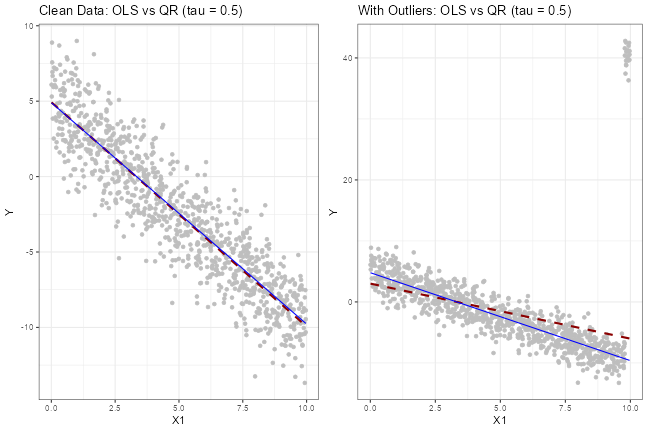
\includegraphics[width=0.8\linewidth]{ADR_project_draft_files/figure-latex/unnamed-chunk-2-1} 

}

\caption{OLS vs QR under high leverage outliers}\label{fig:unnamed-chunk-2}
\end{figure}

\begin{figure}

{\centering 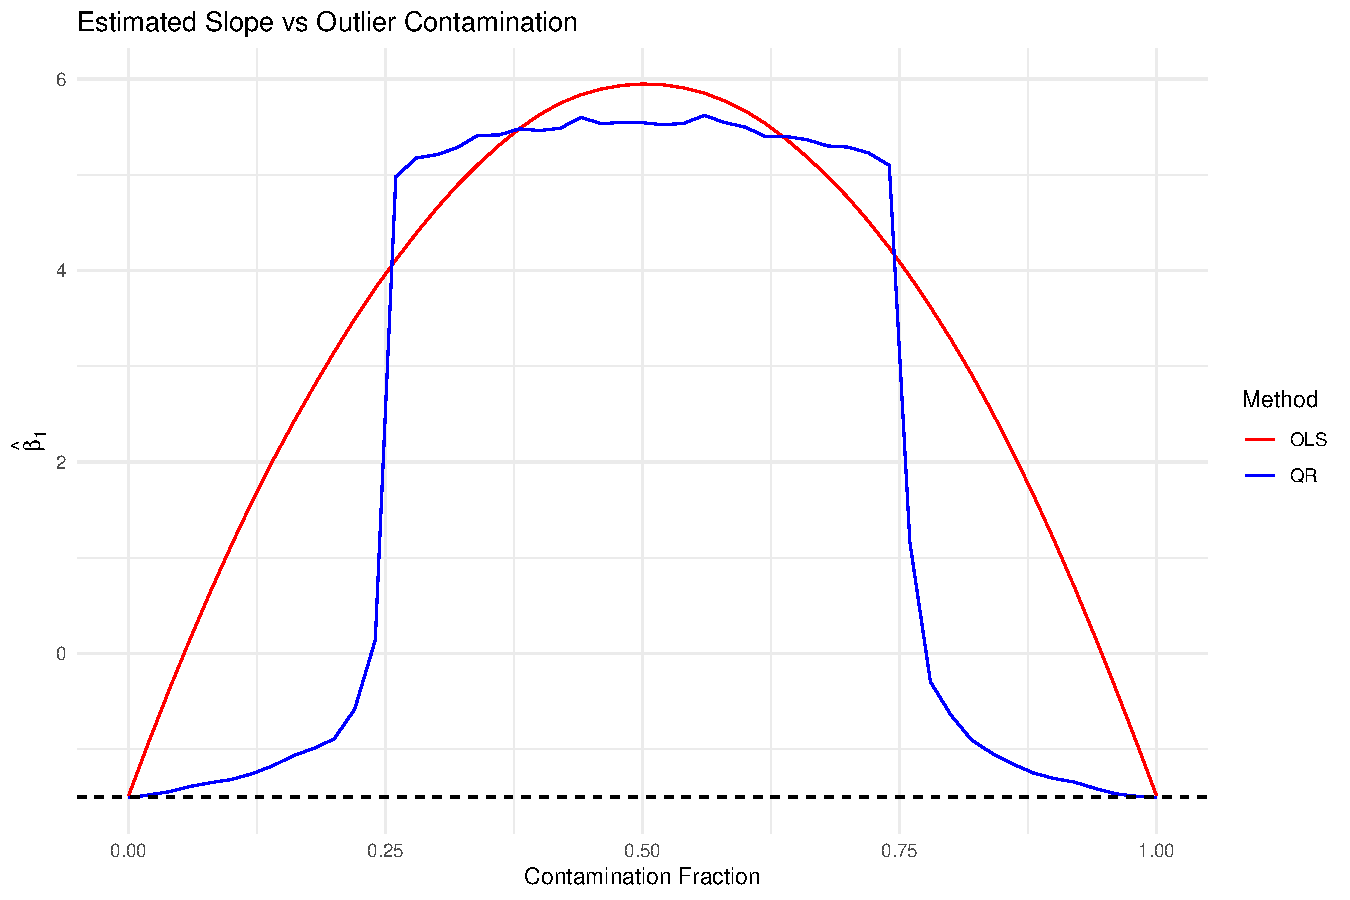
\includegraphics[width=0.8\linewidth]{ADR_project_draft_files/figure-latex/unnamed-chunk-3-1} 

}

\caption{OLS vs QR under random outliers}\label{fig:unnamed-chunk-3}
\end{figure}

Figure 2 illustrates how non high-leverage outliers affect slope estimates. In this specific scenario, both Ordinary Least Squares (OLS) and Quantile Regression (QR) produce similar results, with OLS showing minimal sensitivity to the outliers. This limited impact occurs because the outliers do not occupy high-leverage positions and therefore exert little influence on the slope.

As shown in Table 1, the evaluation of all scenarios reveals that OLS and Quantile Regression (QR) at τ = 0.5 perform similarly under clean data conditions. However, when outliers are introduced, OLS exhibits significant bias, particularly in the slope, and its error metrics (MAE and RMSE), computed on the clean data, deteriorate.
In the case of high leverage outliers, where extreme X values exert a large influence on the model, OLS shows substantial bias in the slope, while QR remains stable with minimal bias and consistent error metrics.
For random outliers, where extreme Y values are scattered across the data, OLS again shows deterioration in its estimates and error metrics, whereas QR maintains its robustness, demonstrating limited sensitivity to both types of outliers.
This behavior aligns with QR's bounded influence function, which limits the impact of extreme values, unlike OLS, which is more vulnerable to contamination.

\begin{table}[!h]
\centering
\caption{\label{tab:echoFALSE}OLS vs Quantile Regression: Coefficients and Error Metrics under Different Error Structures}
\centering
\begin{tabular}[t]{llrrrrr}
\toprule
Model & Method & Intercept & Slope & Slope\_Bias & MAE & RMSE\\
\midrule
Clean & QR & 4.903 & -1.468 & 0.032 & 1.533 & 1.925\\
Clean & OLS & 4.931 & -1.487 & 0.013 & 1.534 & 1.924\\
Highe Leverage Outliers & QR & 4.791 & -1.442 & 0.058 & 1.534 & 1.930\\
Highe Leverage Outliers & OLS & 3.004 & -0.903 & 0.597 & 2.229 & 2.746\\
Random Outliers & QR & 4.935 & -1.468 & 0.032 & 1.533 & 1.927\\
\addlinespace
Random Outliers & OLS & 5.917 & -1.484 & 0.016 & 1.726 & 2.168\\
\bottomrule
\end{tabular}
\end{table}

\begin{figure}

{\centering 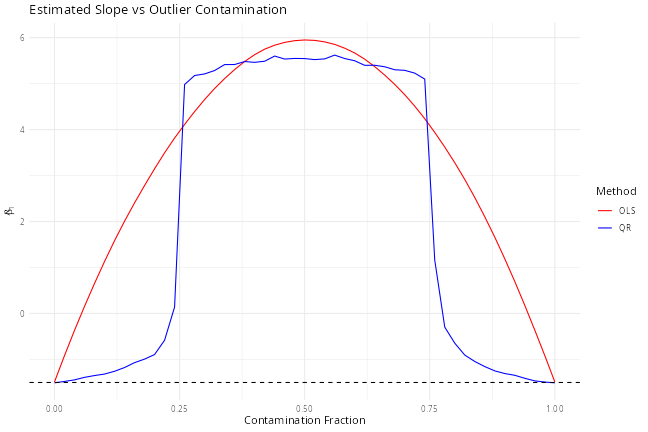
\includegraphics[width=0.8\linewidth]{ADR_project_draft_files/figure-latex/unnamed-chunk-4-1} 

}

\caption{Estimated slope vs outlier contamination}\label{fig:unnamed-chunk-4}
\end{figure}

Figure 3 shows Ordinary Least Squares (OLS) slope immediately degrading under high leverage outlier contamination due to its sensitivity to squared errors. Quantile Regression (QR) initially resists, maintaining a stable slope by focusing on the median. However, QR breaks down beyond a critical outlier threshold (around 25\%) as outliers then redefine the median.

As contamination approaches 100\%, both OLS and QR exhibit a similar pattern: the original data points become the new \enquote{outliers.} Consequently, the estimated slope for both methods may revert to a value resembling the original slope. Critically, this is not a true recovery for either, as the entire fitted line has significantly shifted, now reflecting the characteristics of the overwhelming majority of (initially outlying) data points.

\subsubsection{Heteroscedasticity}\label{heteroscedasticity}

Beyond outlier robustness, Quantile Regression also excels in capturing distributional changes. This subsection demonstrates its effectiveness in handling heteroscedasticity, where the response variable's spread is dependent on the predictors.

In Figure 4 illustrates how the estimated slope coefficient in quantile regression varies across quantile levels \(\tau \in (0.1, 0.9)\) in a heteroskedastic setting. The increasing slope as \(\tau\) increases reflects the presence of conditional heteroskedasticity: higher quantiles are associated with greater dispersion in the response variable \(Y\), which alters the marginal effect of \(X_1\) across the conditional distribution. Quantile regression estimates \(\beta_1(\tau)\) independently for each \(\tau\), capturing variation in the conditional distribution of \(Y\) while the slope of OLS remains constant because it targets the conditional mean and assumes homoscedasticity.

\begin{figure}[h]

{\centering 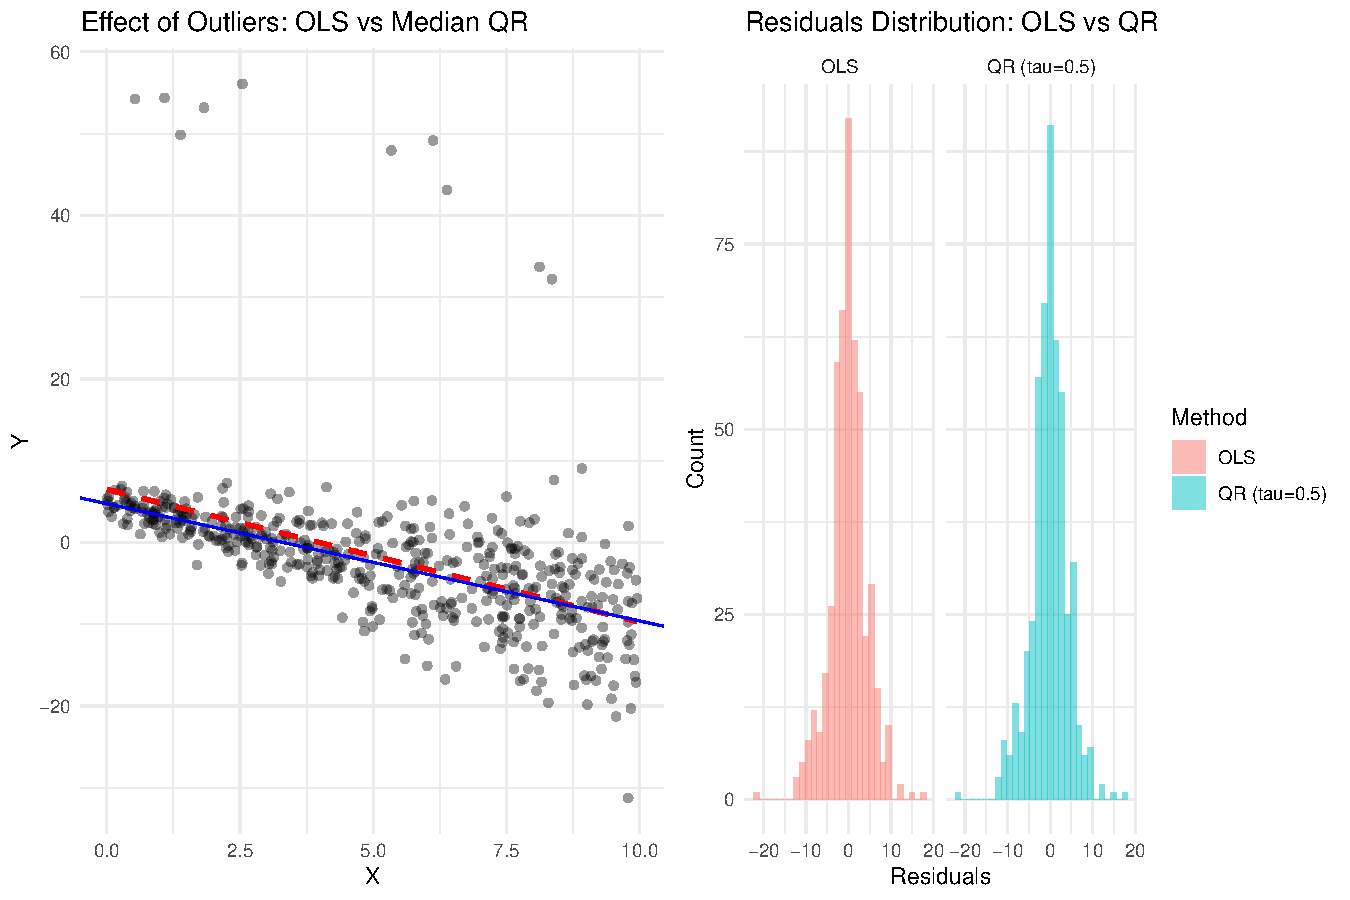
\includegraphics[width=0.8\linewidth]{ADR_project_draft_files/figure-latex/unnamed-chunk-5-1} 

}

\caption{Slope vs Quantile for heteroskedastic data}\label{fig:unnamed-chunk-5}
\end{figure}

\section{Discussion \& Conclusions}\label{discussion-conclusions}

This report has compared ordinary least squares (OLS) and quantile regression (QR) for modeling linear relationships, focusing on scenarios where classical OLS assumptions are violated. Through controlled simulations, we demonstrated two primary advantages of QR. Firstly, QR (\(\tau=0.5\)) exhibits significant \textbf{robustness to outliers}, providing stable and reliable coefficient estimates even under contamination with high-leverage points, a condition where OLS estimates suffered severe bias (as shown in Figure 1 and Table 1. This resilience stems from QR's use of the check loss function, which minimizes absolute deviations rather than squared deviations.

Second, QR effectively models distributional heterogeneity, capturing how predictor effects vary across the conditional distribution. Our heteroscedasticity simulations (Figures 4) revealed trends and spread that OLS, focused solely on the conditional mean, entirely misses. In conclusion, while OLS remains a foundational method for estimating conditional means, quantile regression (QR) provides a more versatile framework---particularly in settings involving outliers, heteroscedasticity, or deviations from Gaussian error structures---by capturing the full conditional distribution and enabling quantile-specific inference.

\textbf{Acknowledgements: This report has been made with a template in R Markdown, taking as example the paper written by \citet{FanLi2001}. CHATGPT has been used for cleaning the code and debugging.}

%----------------------------------------------------------------------------------------
%	REFERENCE LIST
%----------------------------------------------------------------------------------------

\bibliographystyle{apalike}
\makeatletter
% The filename has .bib extension that must be eliminated
\filename@parse{references.bib}
% parse stores the file name in base. Extension starts at the first dot, so don't use dots in file names.
\bibliography{\filename@base}
\makeatother


%----------------------------------------------------------------------------------------

\end{document}
